\chapter{Generazione dei Segnali Secondari}\label{segnali_secondari}

%--------------------------------------------------------------------------------------------

Ora si passa a estrarre i segnali mancanti da quelli principali generati al capitolo \ref{segnali_principali}.

%--------------------------------------------------------------------------------------------

\section{Dente di Sega}

%--------------------------------------------------------------------------------------------

Il più facile da generare è sicuramente il dente di sega in quanto tutto quello che serve è un
semplice amplificatore invertente con guadagno pari a uno.

\begin{figure}[H]
    \centering
    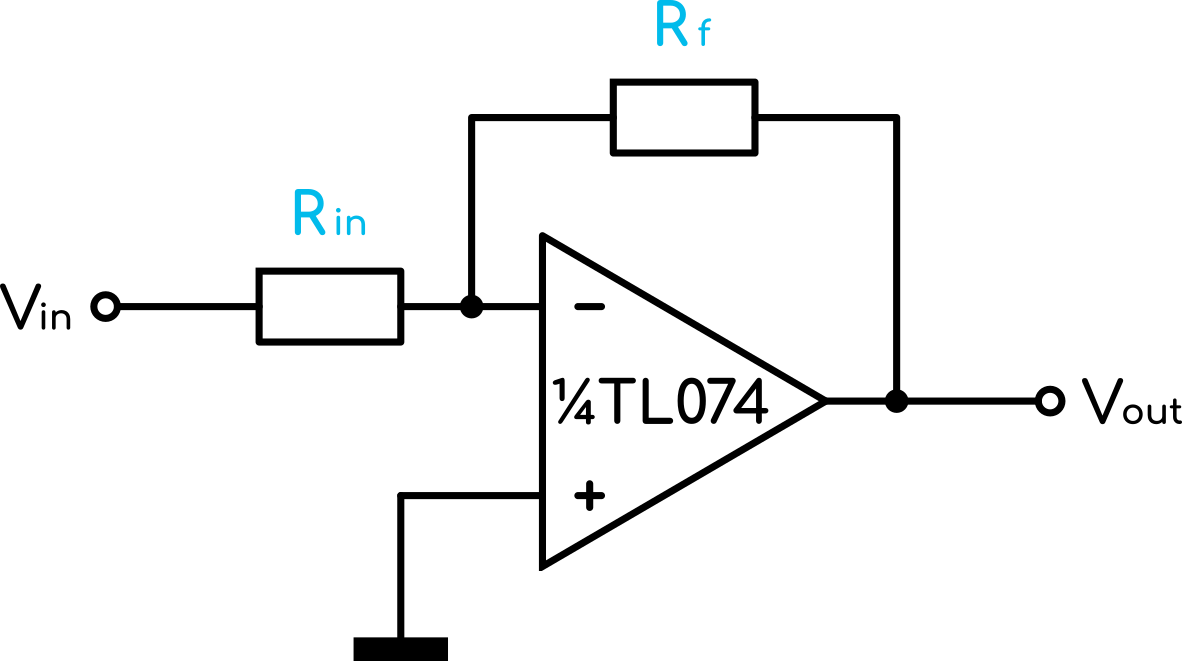
\includegraphics{circuits/inverting_amp_circuit.png}
    \caption{Schema dell'amplificatore invertente}
    \label{inverting_amp_circuit}
\end{figure}

Come sempre l'operazionale utilizzato è un TL074.

Dalla relazione dell'amplificatore invertente vediamo che per avere un guadagno unitario si
deve porre la resistenza di feedback uguale a quella di ingresso, $R_{in}=R_f$.

\begin{equation}
    V_{out}=-V_{in}\frac{R_{in}}{R_f}=-V_{in}\ [V]
\end{equation}

Questo è quanto ottenuto in uscita:

\begin{figure}[H]
    \centering

    \begin{subfigure}{.5\textwidth}
        \centering
        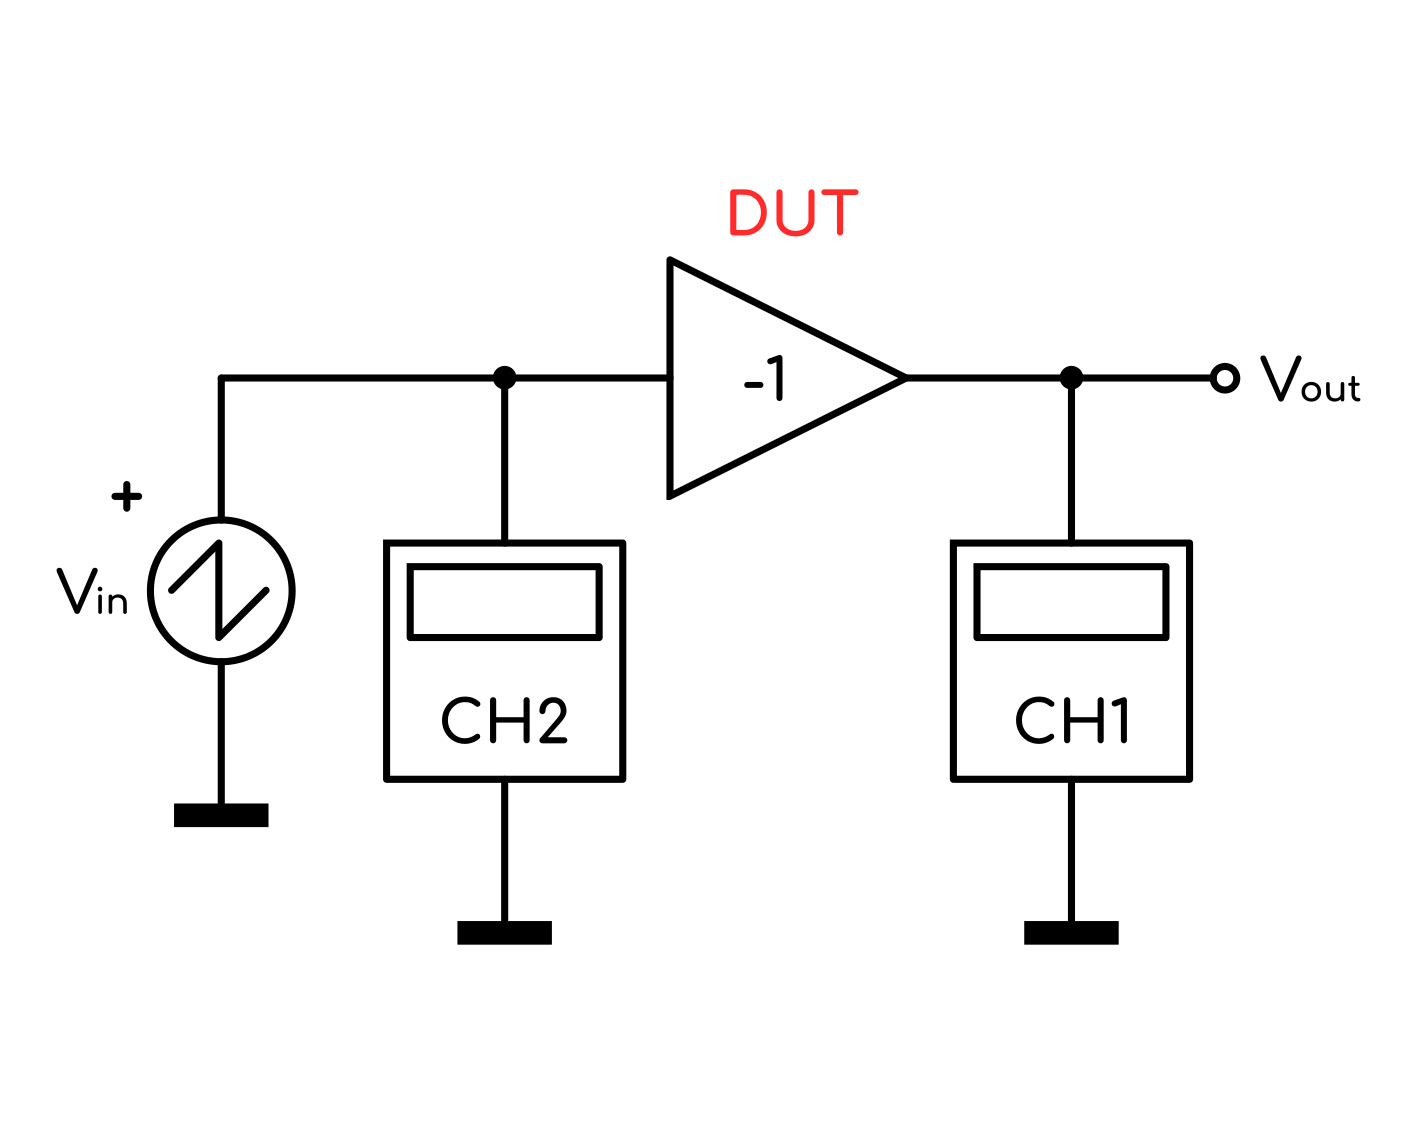
\includegraphics{block_diagrams/mis_saw.png}
        \caption{Setup di misura}
        \label{mis_saw}
    \end{subfigure}%
    \begin{subfigure}{.5\textwidth}
        \centering
        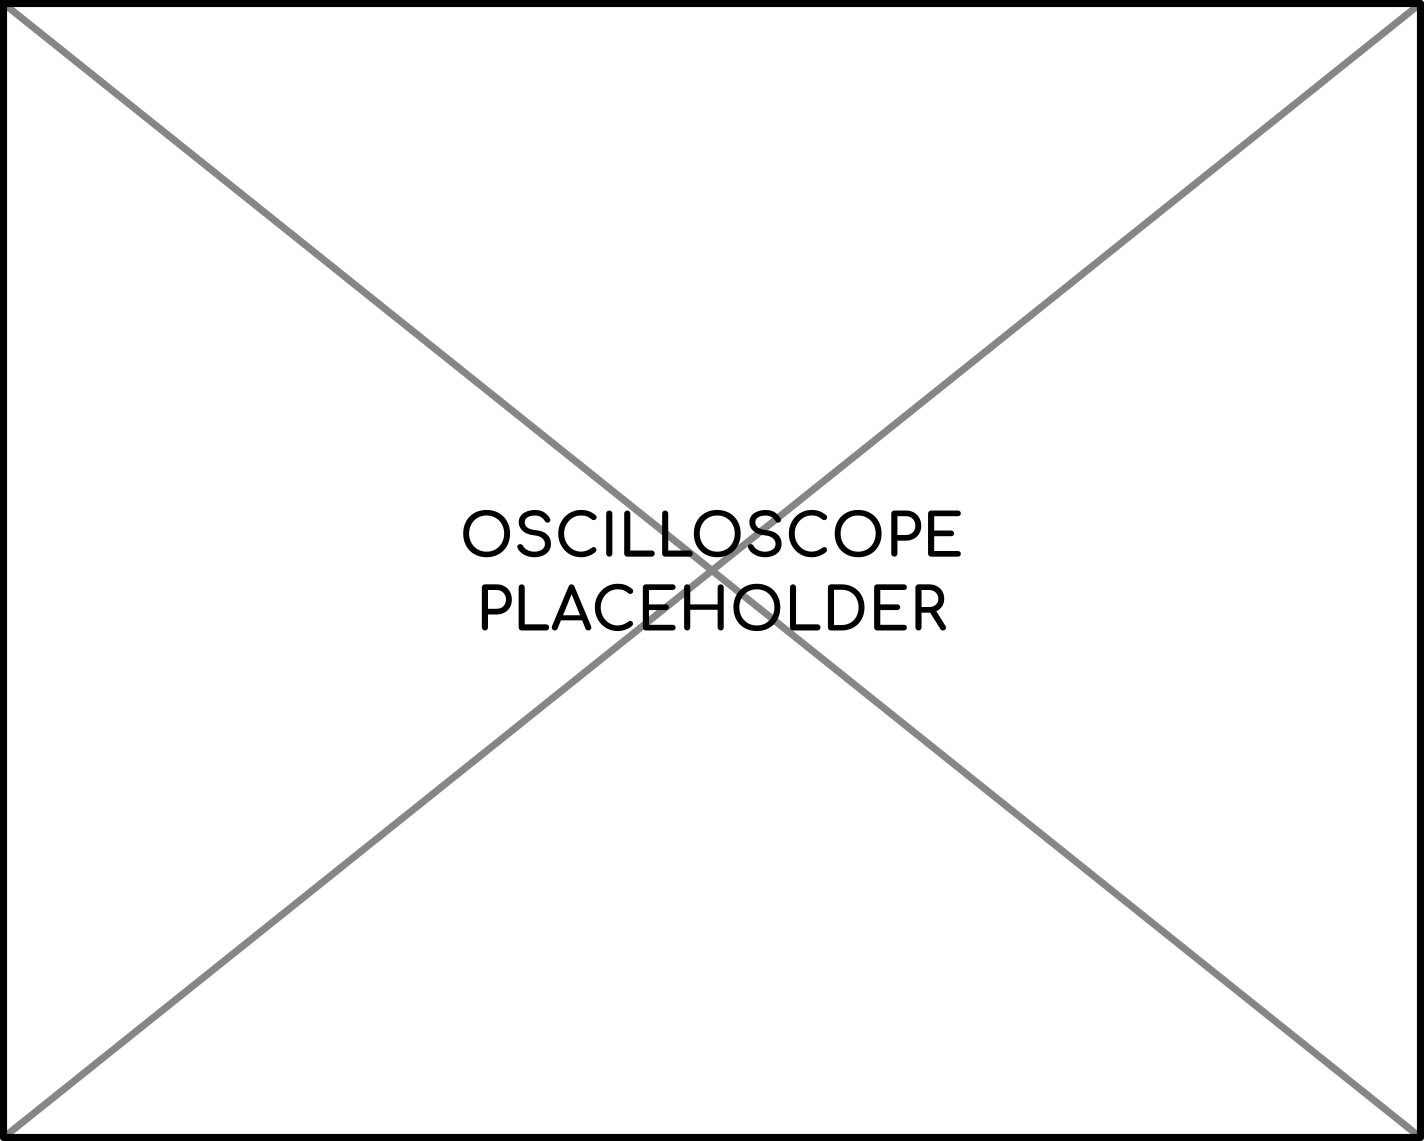
\includegraphics{misc/oscilloscope_placeholder.png}
        \caption{Acquisizione dell'onda ottenuta}
        \label{acq_saw}
    \end{subfigure}

    \caption{Misura del segnale a dente di sega}
\end{figure}

%--------------------------------------------------------------------------------------------

\section{Onda Quadra}

%--------------------------------------------------------------------------------------------

Anche l'onda quadra risulta piuttosto semplice da generare, in quanto è necessario solo
aggiungere un offset e un guadagno al segnale utilizzato per il pilotaggio del contatore
bidirezionale, ovvero $U/D$. Tale segnale infatti ha già forma e frequenza desiderate, è però
compresa solo tra $0\ V$ e $+5\ V$, e si deve estendere fino a $-5\ V$.
Si utilizza quindi un altro amplificatore invertente con riferimento diverso da massa, lo
schema è il seguente:

\begin{figure}[H]
    \centering
    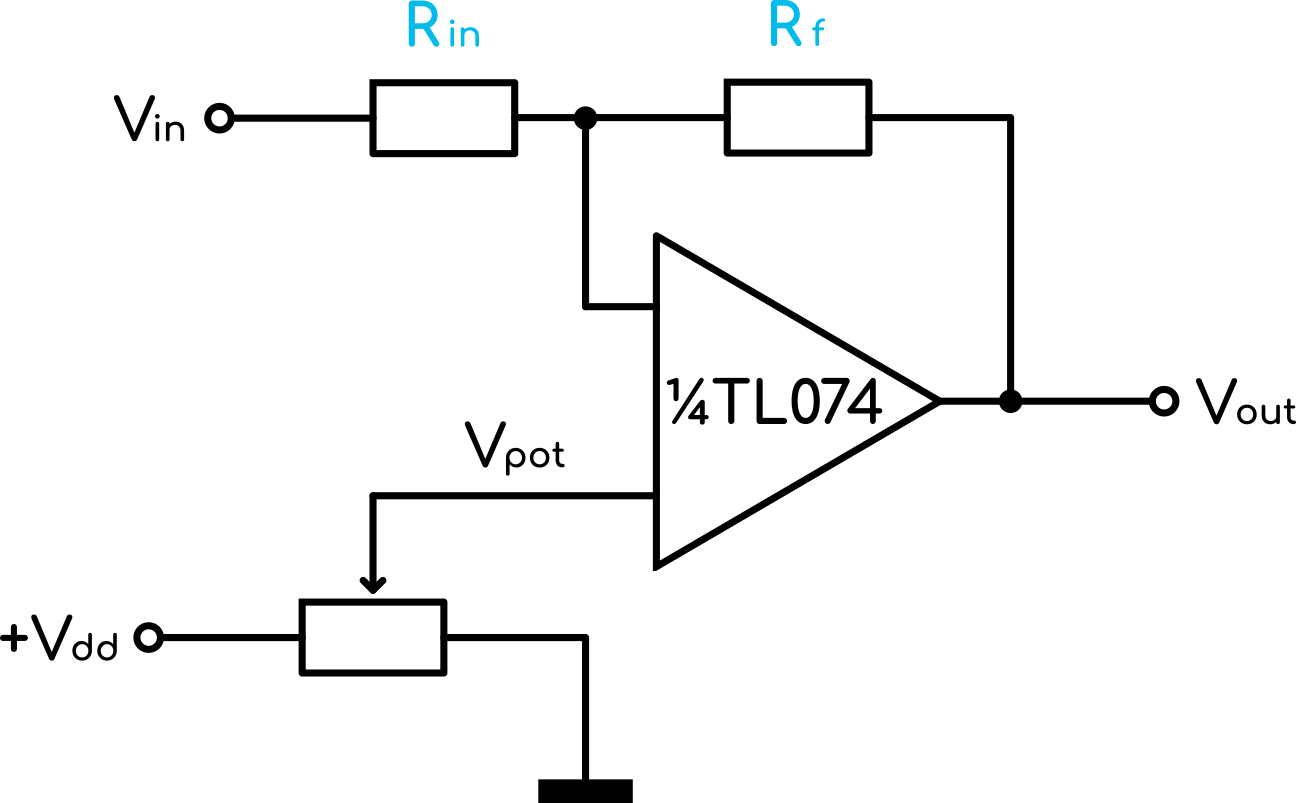
\includegraphics{circuits/inverting_amp_offset_circuit.png}
    \caption{Schema dell'amplificatore invertente con offset ($+V_{dd}=+5\ V$)}
    \label{inverting_amp_offset_circuit}
\end{figure}

in cui si utilizzano due trimmer per la regolazione precisa di guadagno e offset.

La relazione ingresso/uscita è:

\begin{equation}
    V_{out}=V_{pot}\left(1+\frac{R_f}{R_{in}}\right)-V_{in}\frac{R_f}{R_{in}}\ [V]
\end{equation}

dove si vede chiaramente che $-\frac{R_f}{R_{in}}$ è il guadagno e $V_{pot}\left(1+\frac{R_f}{R_{in}}\right)$
l'offset.

La forma d'onda osservata in uscita è quindi la seguente:

\begin{figure}[H]
    \centering

    \begin{subfigure}{.5\textwidth}
        \centering
        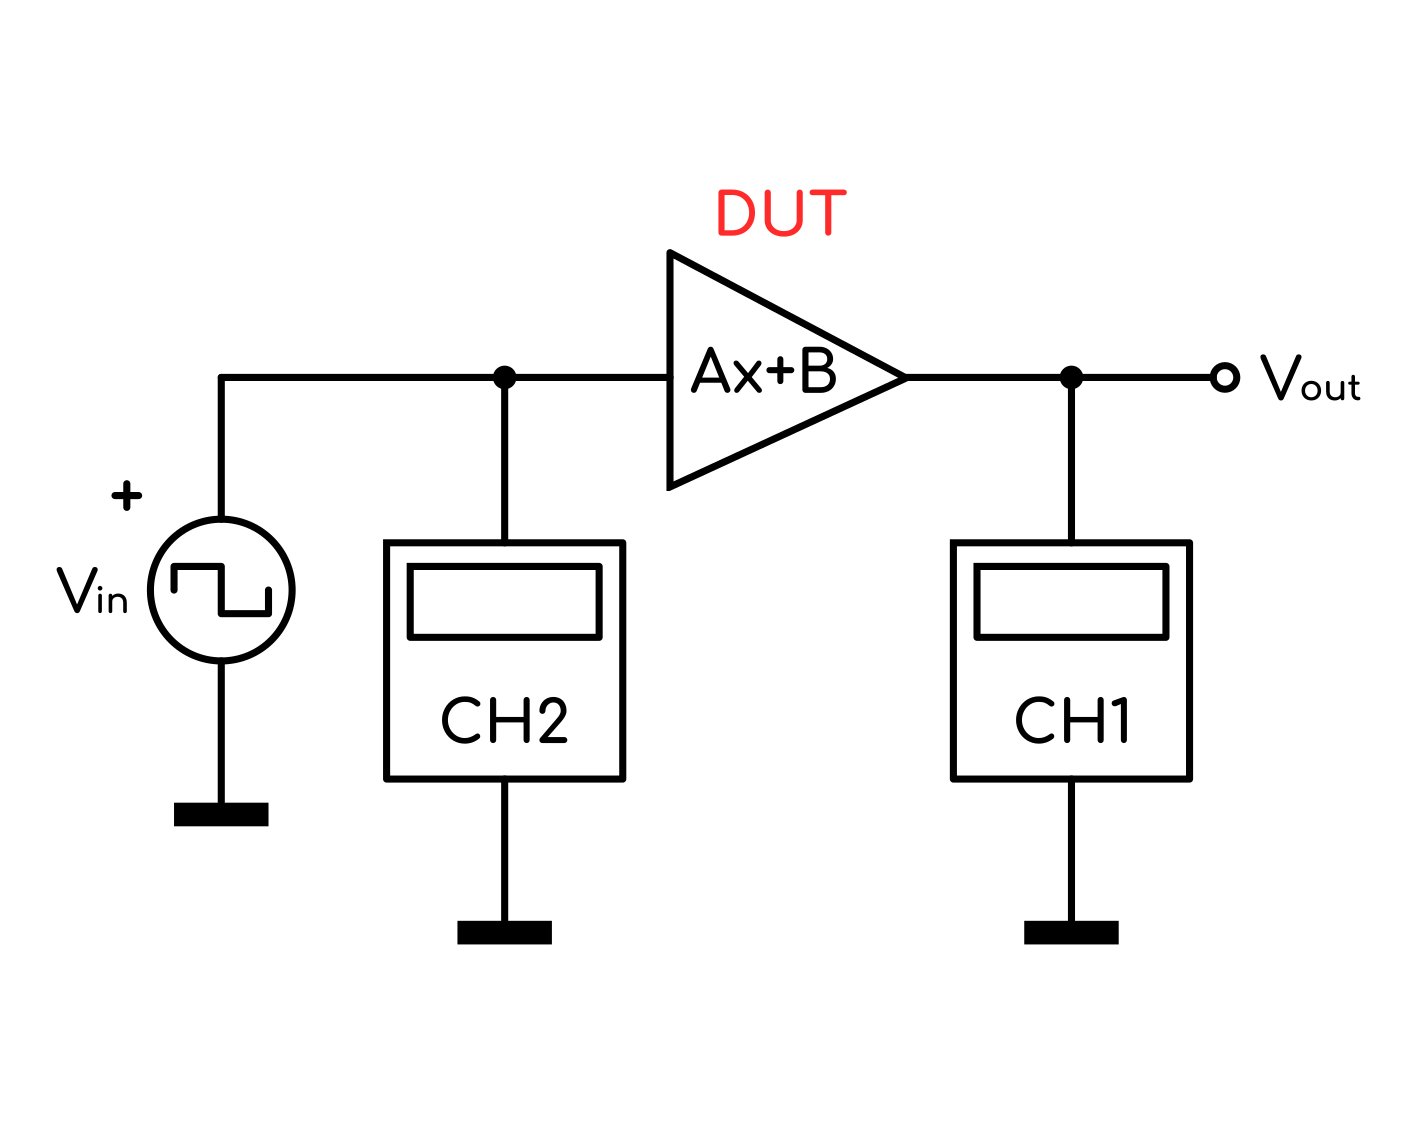
\includegraphics{block_diagrams/mis_square.png}
        \caption{Setup di misura}
        \label{mis_square}
    \end{subfigure}%
    \begin{subfigure}{.5\textwidth}
        \centering
        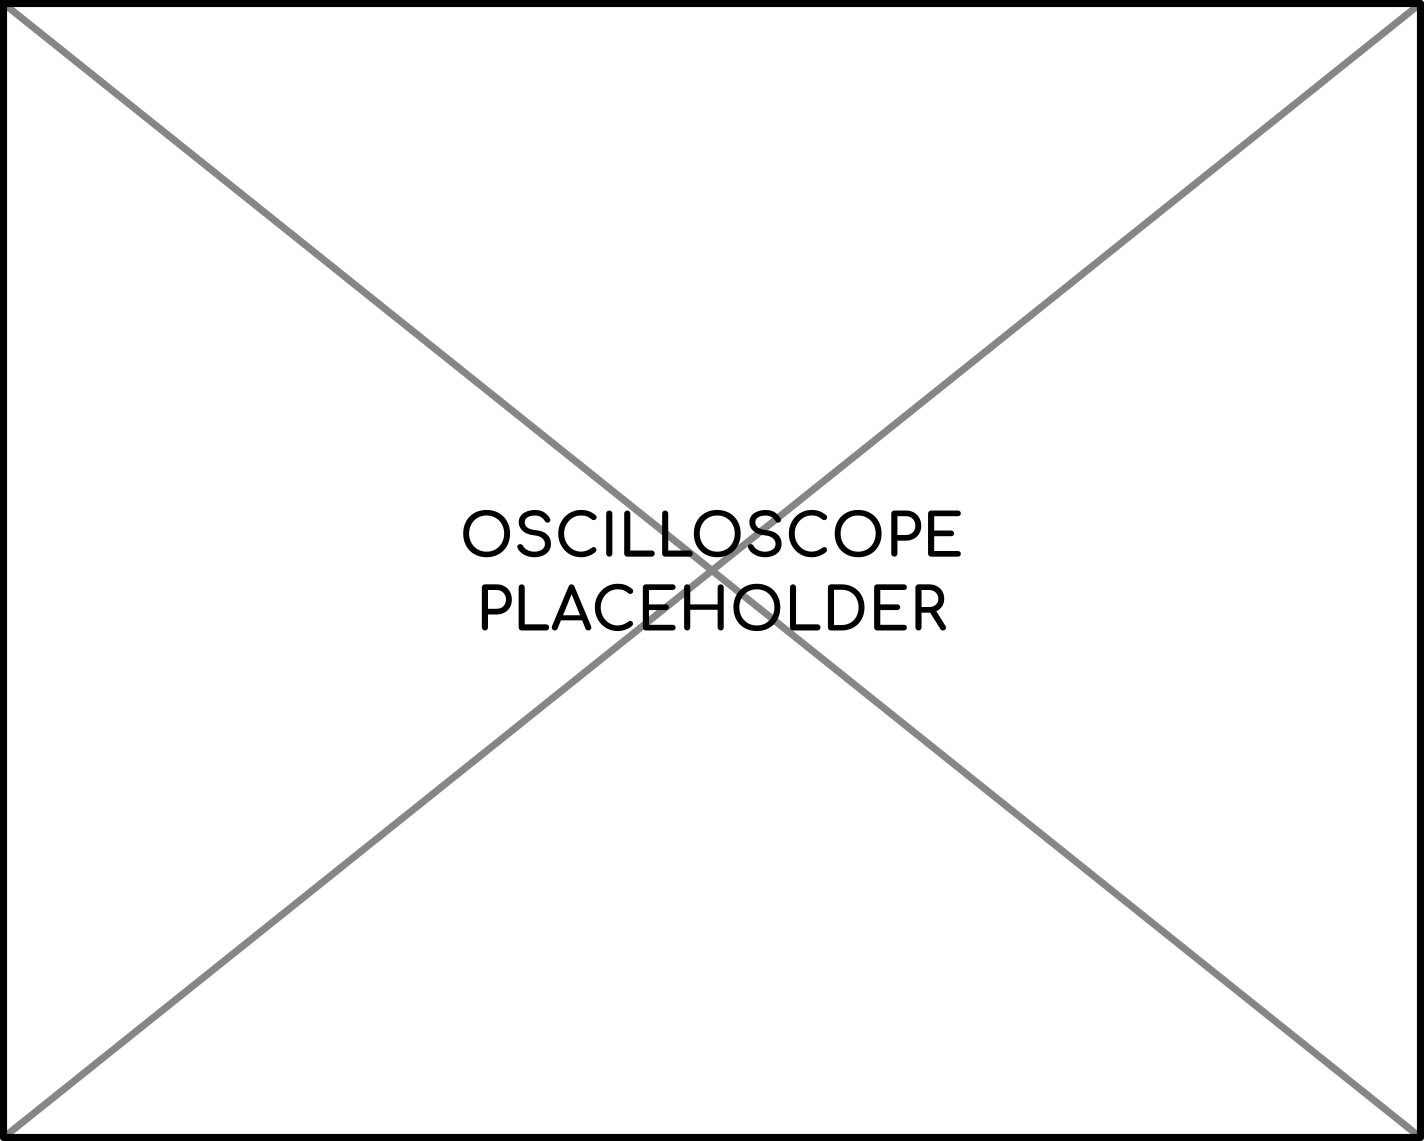
\includegraphics{misc/oscilloscope_placeholder.png}
        \caption{Acquisizione dell'onda ottenuta}
        \label{acq_square}
    \end{subfigure}

    \caption{Misura del segnale a onda quadra ottenuto}
\end{figure}

%--------------------------------------------------------------------------------------------

\section{Impulso}

%--------------------------------------------------------------------------------------------

Per quanto riguarda l'impulso invece, facciamo uso del segnale $RCO$ ricavato al capitolo
\ref{segnali_principali}, figura \ref{ramp_counter_circuit}. Tale segnale viene portato in
ingresso ad un circuito monostabile realizzato con un celebre NE555 \cite{ne555} che si
occuperà di aumentare la durata dell'impulso per valori di frequenza più elevati. Lo schema
utilizzato, è riportato in figura \ref{monostable_circuit} e viene preso da pg.10 del
datasheet.

\begin{figure}[H]
    \centering
    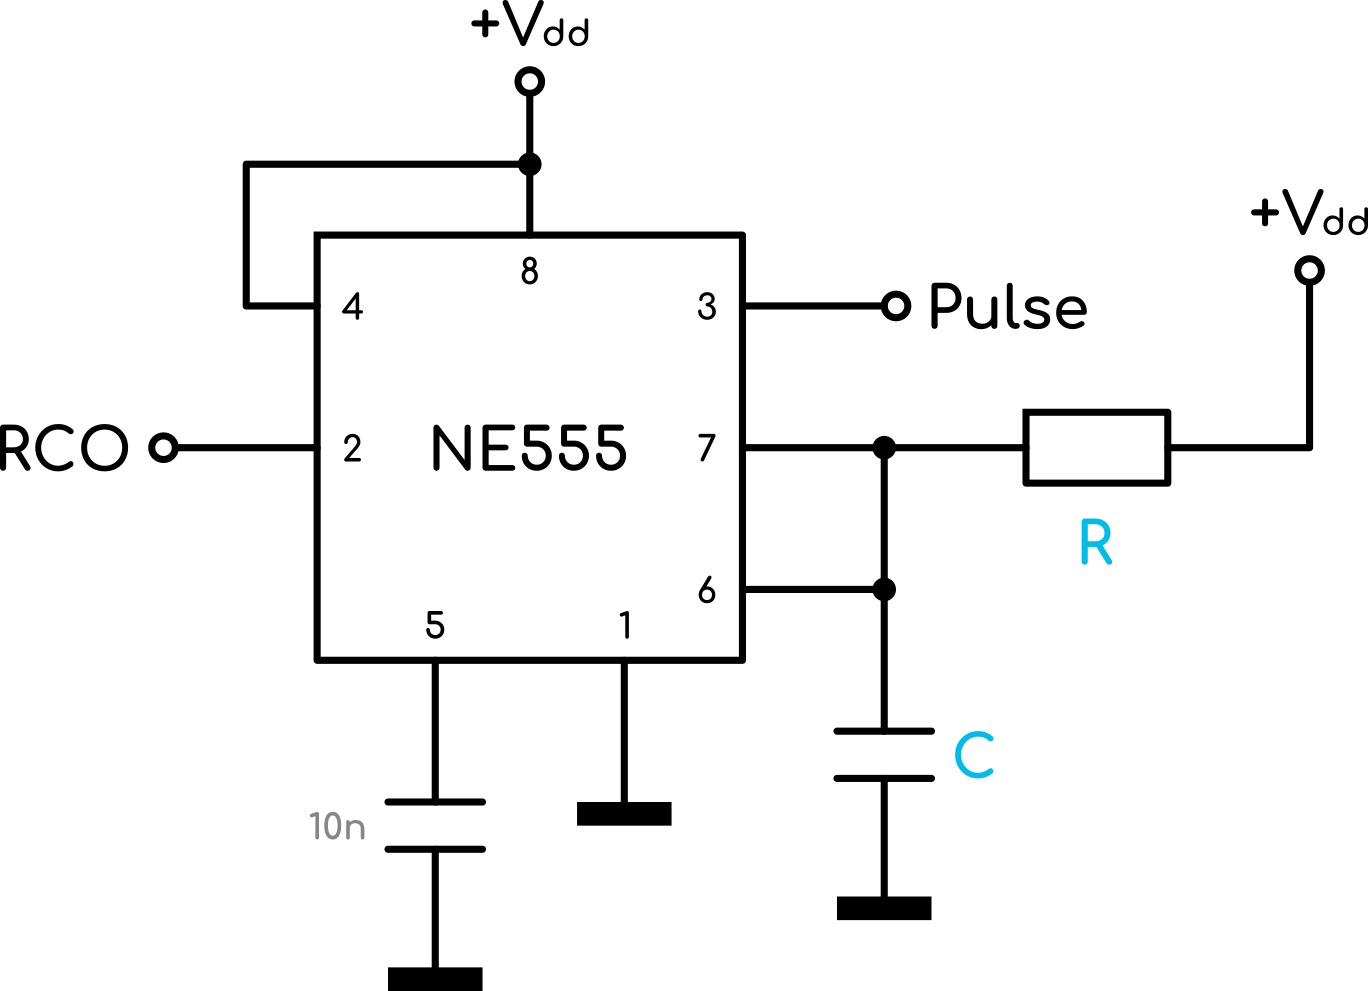
\includegraphics{circuits/monostable_circuit.png}
    \caption{Schema circuito monostabile ($+V_{dd}=+5\ V$)}
    \label{monostable_circuit}
\end{figure}

La relazione sul periodo dell'impulso in uscita (anch'essa ricavata dal datasheet) è la
seguente:

\begin{equation}
    t_w=1.1RC\ [s]
\end{equation}

Si scelgono $R=10\ k\Omega$ e $C=100\ pF$ per ottenere un periodo di impulso di circa
$1.1\ \mu s$.

Si osservano quindi le forme d'onda così ottenute:

\begin{figure}[H]
    \centering
    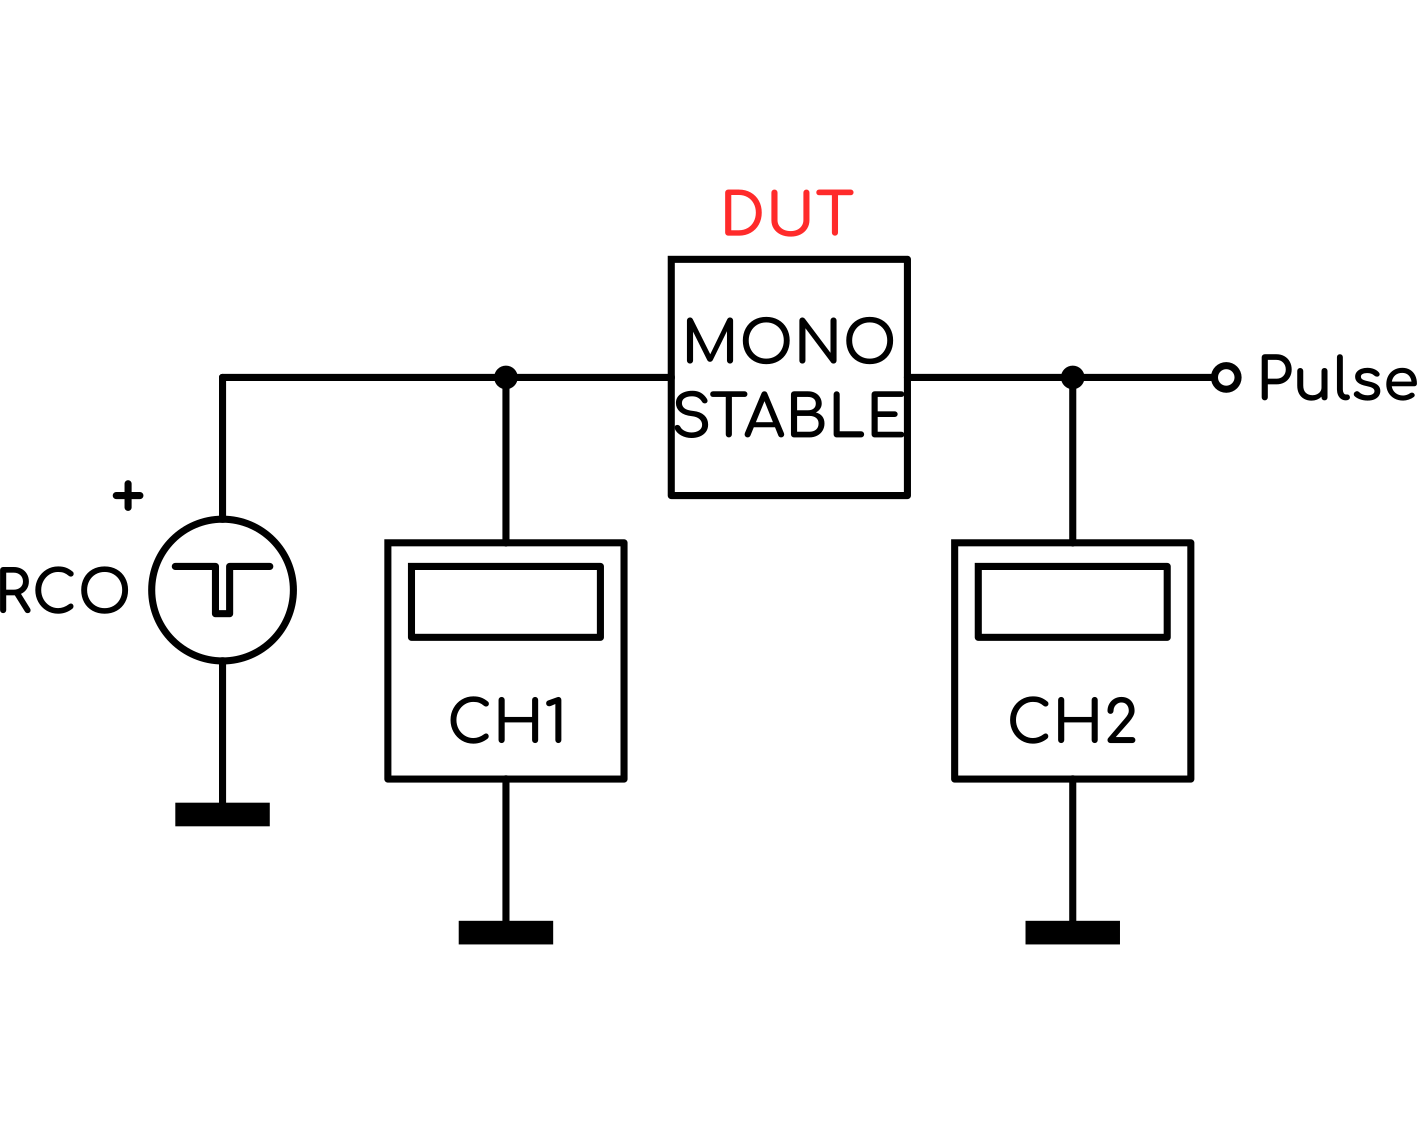
\includegraphics{block_diagrams/mis_monostable.png}
    \caption{Setup di misura del circuito monostabile}
    \label{mis_monostable}
\end{figure}

\begin{figure}[H]
    \centering

    \begin{subfigure}{.5\textwidth}
        \centering
        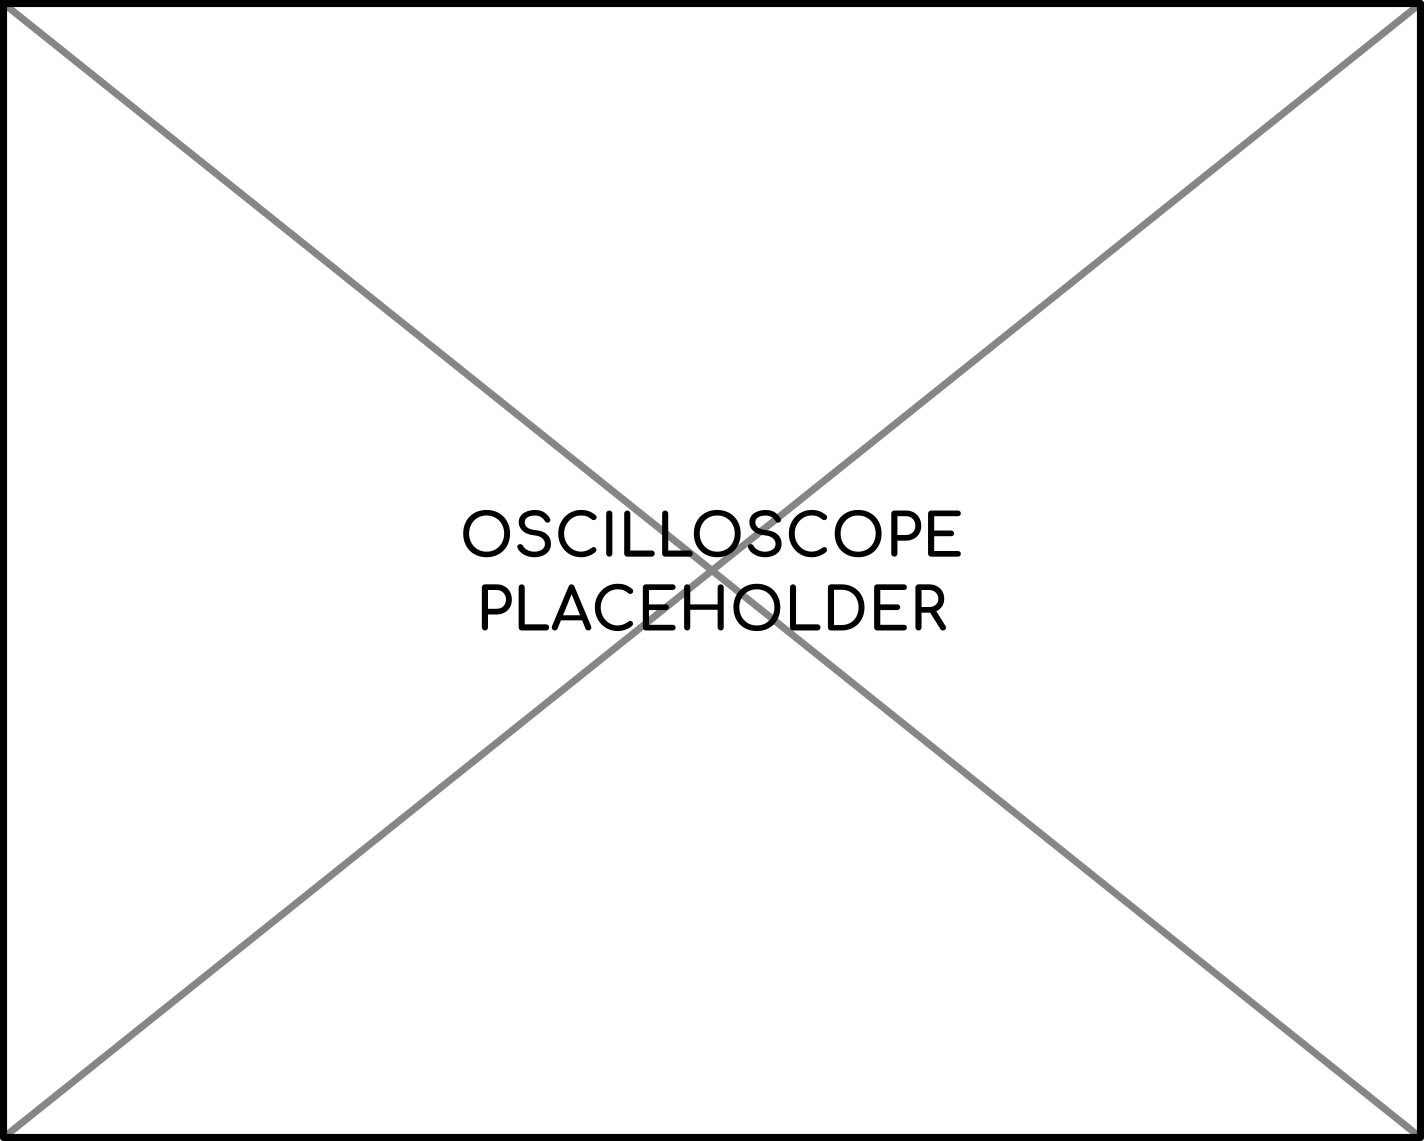
\includegraphics{misc/oscilloscope_placeholder.png}
        \caption{$V_{in}=+2\ V$}
        \label{acq_monostable_2V}
    \end{subfigure}%
    \begin{subfigure}{.5\textwidth}
        \centering
        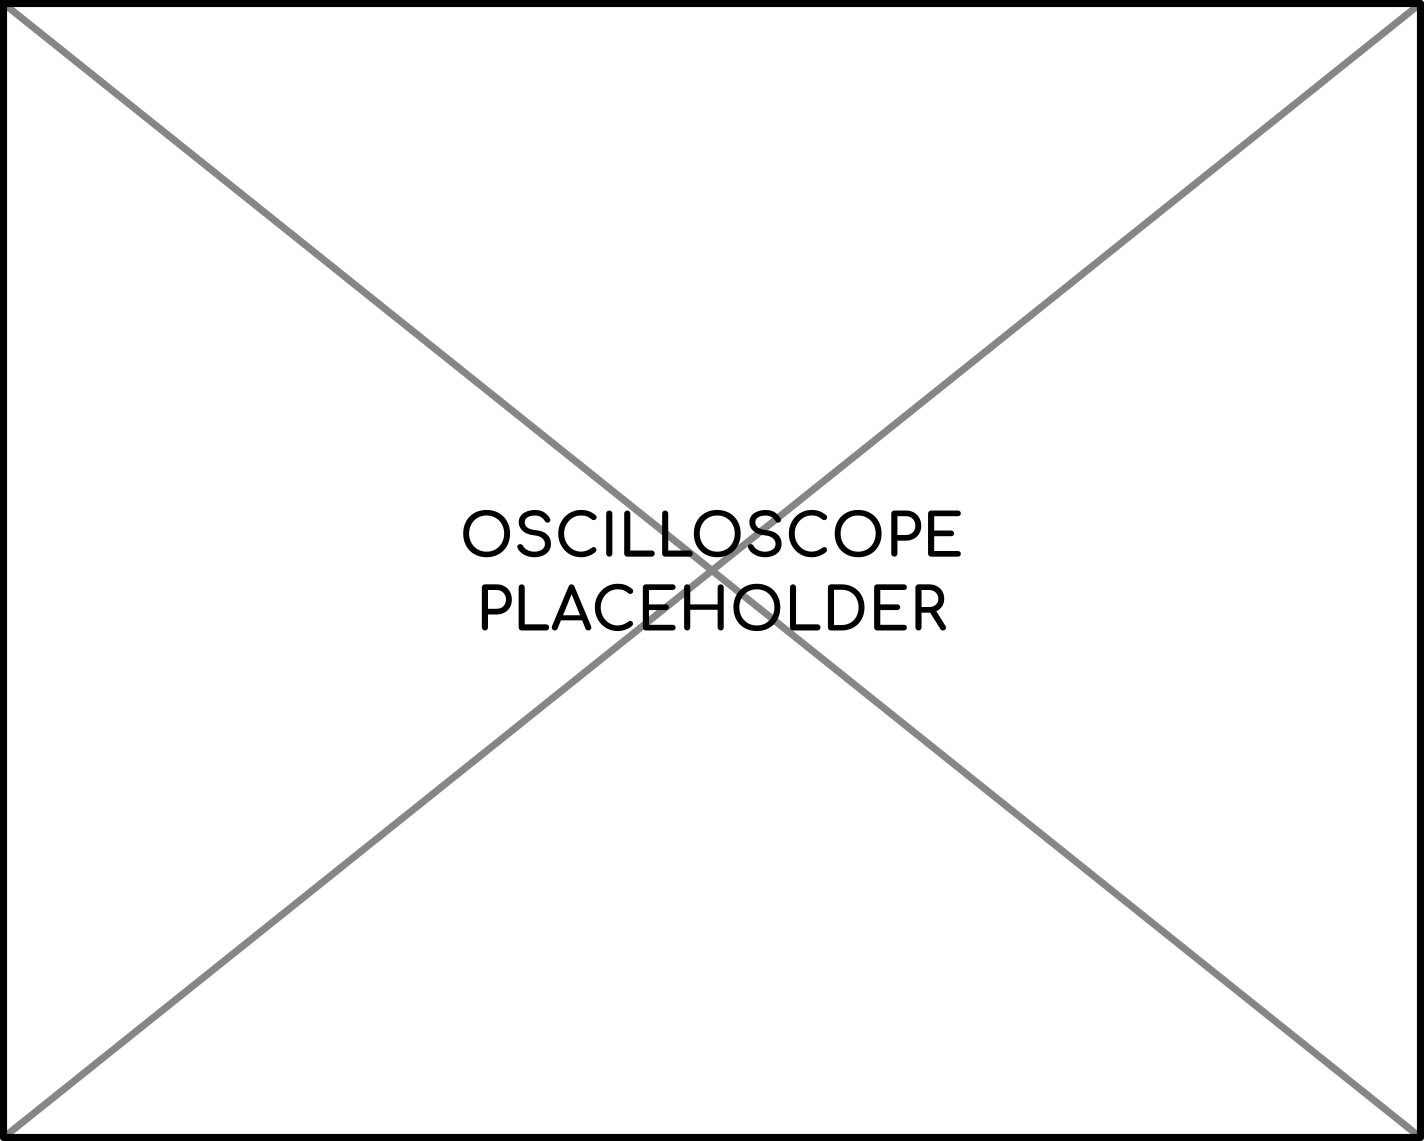
\includegraphics{misc/oscilloscope_placeholder.png}
        \caption{$V_{in}=+8\ V$}
        \label{acq_monostable_8V}
    \end{subfigure}

    \caption{Acquisizioni dei segnali $RCO$ e $Pulse$ per diversi valori di $V_{in}$}
    \label{mis_pulse}
\end{figure}

%--------------------------------------------------------------------------------------------

\section{Sinusoide}

%--------------------------------------------------------------------------------------------

Infine, l'onda più complicata da generare, ma più semplice per caratteristiche è la sinusoide.
Un modo piuttosto semplice per generarla sarebbe filtrare al massimo una qualsiasi delle onde
già generate, e lasciare solo l'armonica fondamentale. Tuttavia questo metodo risulta scomodo
se la frequenza del segnale varia in un ampio spettro, come appunto nel nostro caso, perchè la
frequenza di taglio del filtro dovrebbe seguire di pari passo quella dell'oscillatore.

La soluzione utilizzata quindi è un circuito con guadagno variabile in base al livello di
tensione fornito in ingresso, realizzato con un operazionale e dei diodi, sia normali che di
tipo zener, i quali si occupano di modificare la resistenza di feedback e quindi il valore di
guadagno dell'amplificatore. A questo circuito viene poi fornito in ingresso il triangolo,
l'onda piu simile alla sinusoide tra quelle generate, e in uscita si ottiene un segnale
abbastanza approssimato di una sinusoide.

% schema elettrico

Per ricavare la relazione ingresso uscita\dots

% relazione e grafico transcaratteristica teorico

Poichè in questo passaggio la tensione massima ottenuta è limitata al valore di breakdown
dei diodi zener nell'anello di feedback, quindi $3.3\ V$ nel nostro caso, è anche necessario
uno stadio amplificatore in cascata per riportare l'onda ai livelli di tensione specificati
dallo standard.

% amplificatore e relazione

Osserviamo quindi l'onda e verifichiamo quanto risulta buona come approssimazione:

% circuito di misura

\begin{figure}[H]
    \centering

    \begin{subfigure}{.5\textwidth}
        \centering
        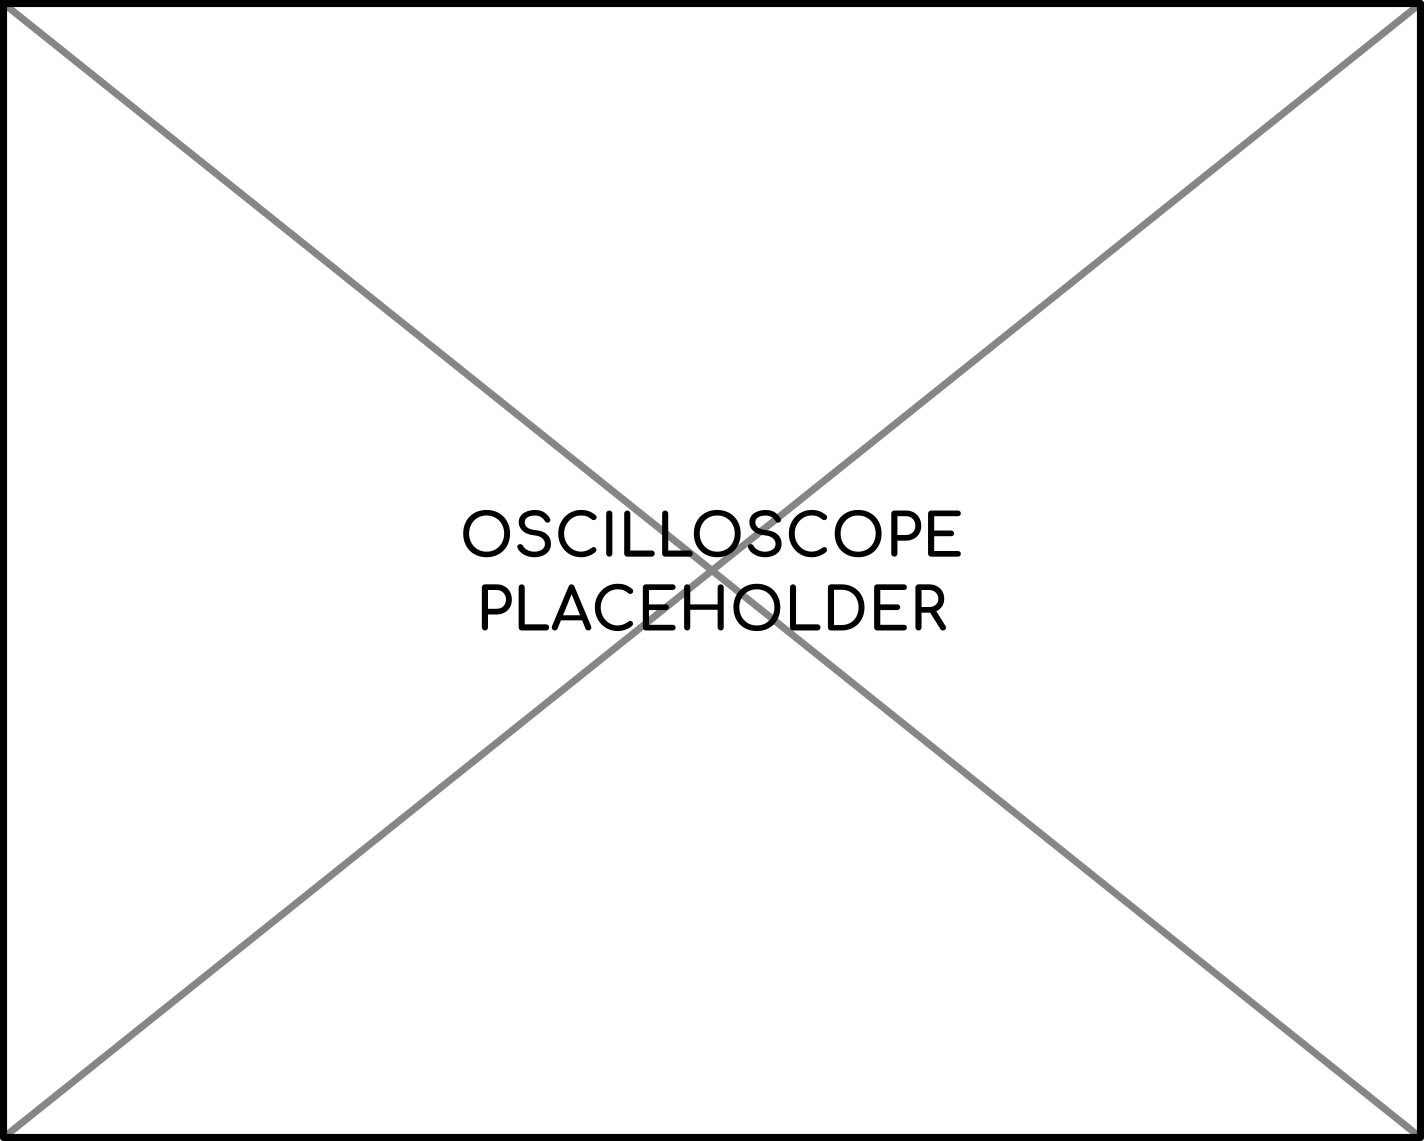
\includegraphics{misc/oscilloscope_placeholder.png}
        \caption{$V_{in}=+2\ V$}
        \label{acq_sine_2V}
    \end{subfigure}%
    \begin{subfigure}{.5\textwidth}
        \centering
        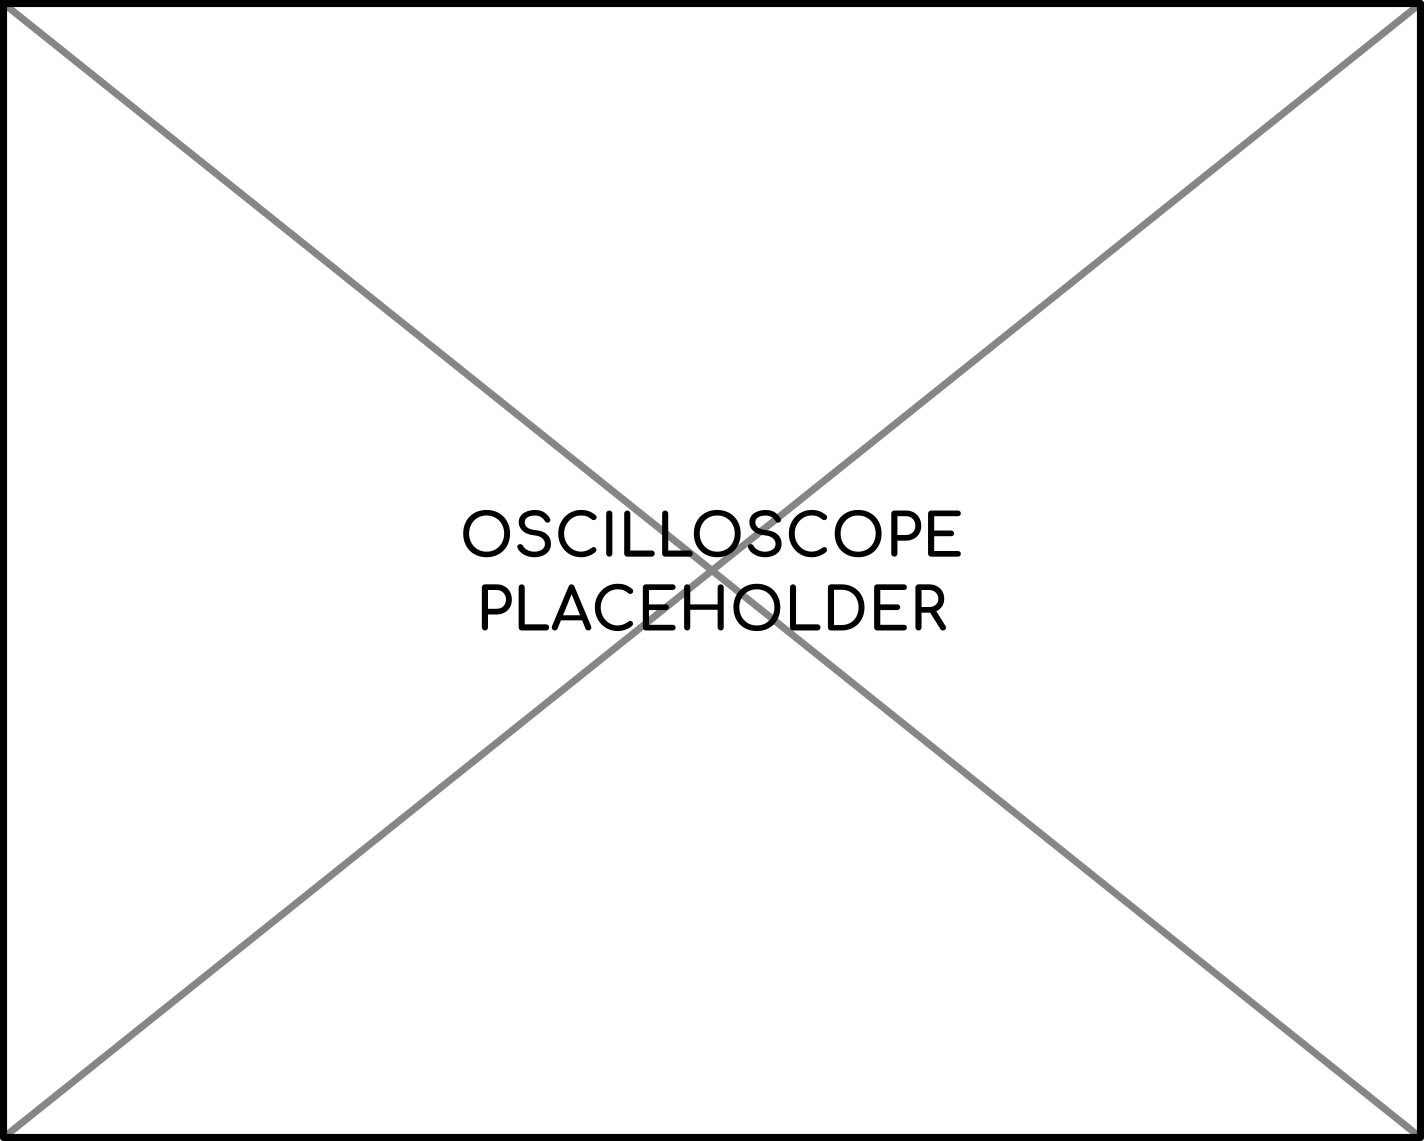
\includegraphics{misc/oscilloscope_placeholder.png}
        \caption{$V_{in}=+8\ V$}
        \label{acq_sine_8V}
    \end{subfigure}
    \begin{subfigure}{.5\textwidth}
        \centering
        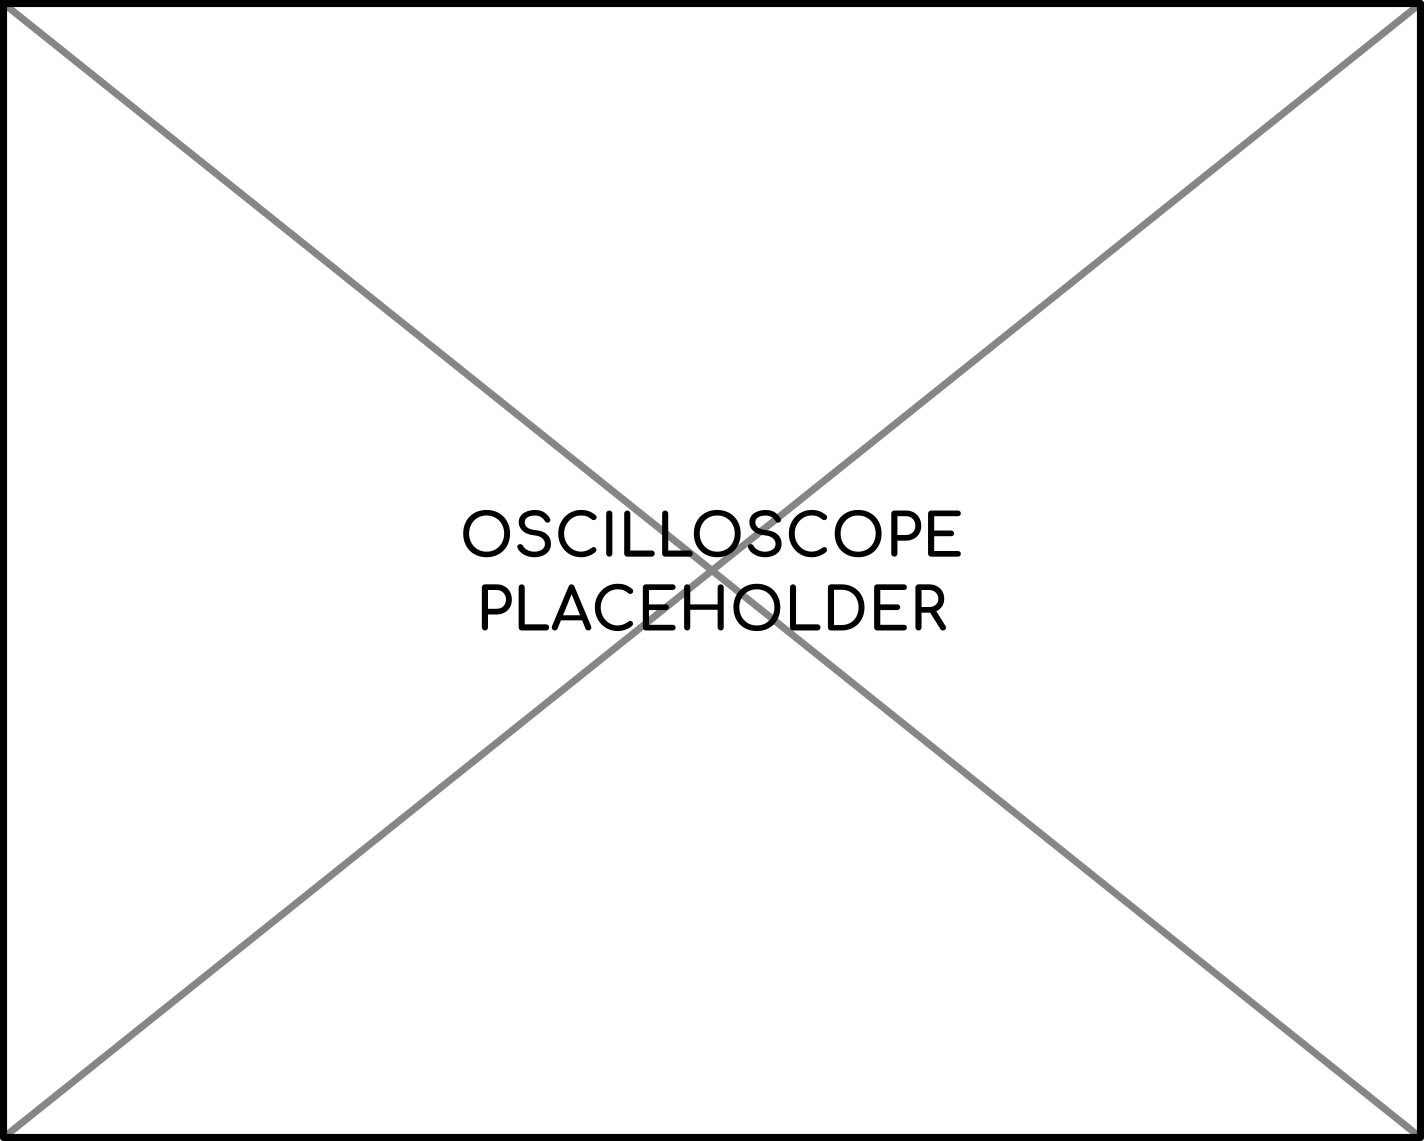
\includegraphics{misc/oscilloscope_placeholder.png}
        \caption{$V_{in}=+2\ V$}
        \label{acq_fourier_2V}
    \end{subfigure}%
    \begin{subfigure}{.5\textwidth}
        \centering
        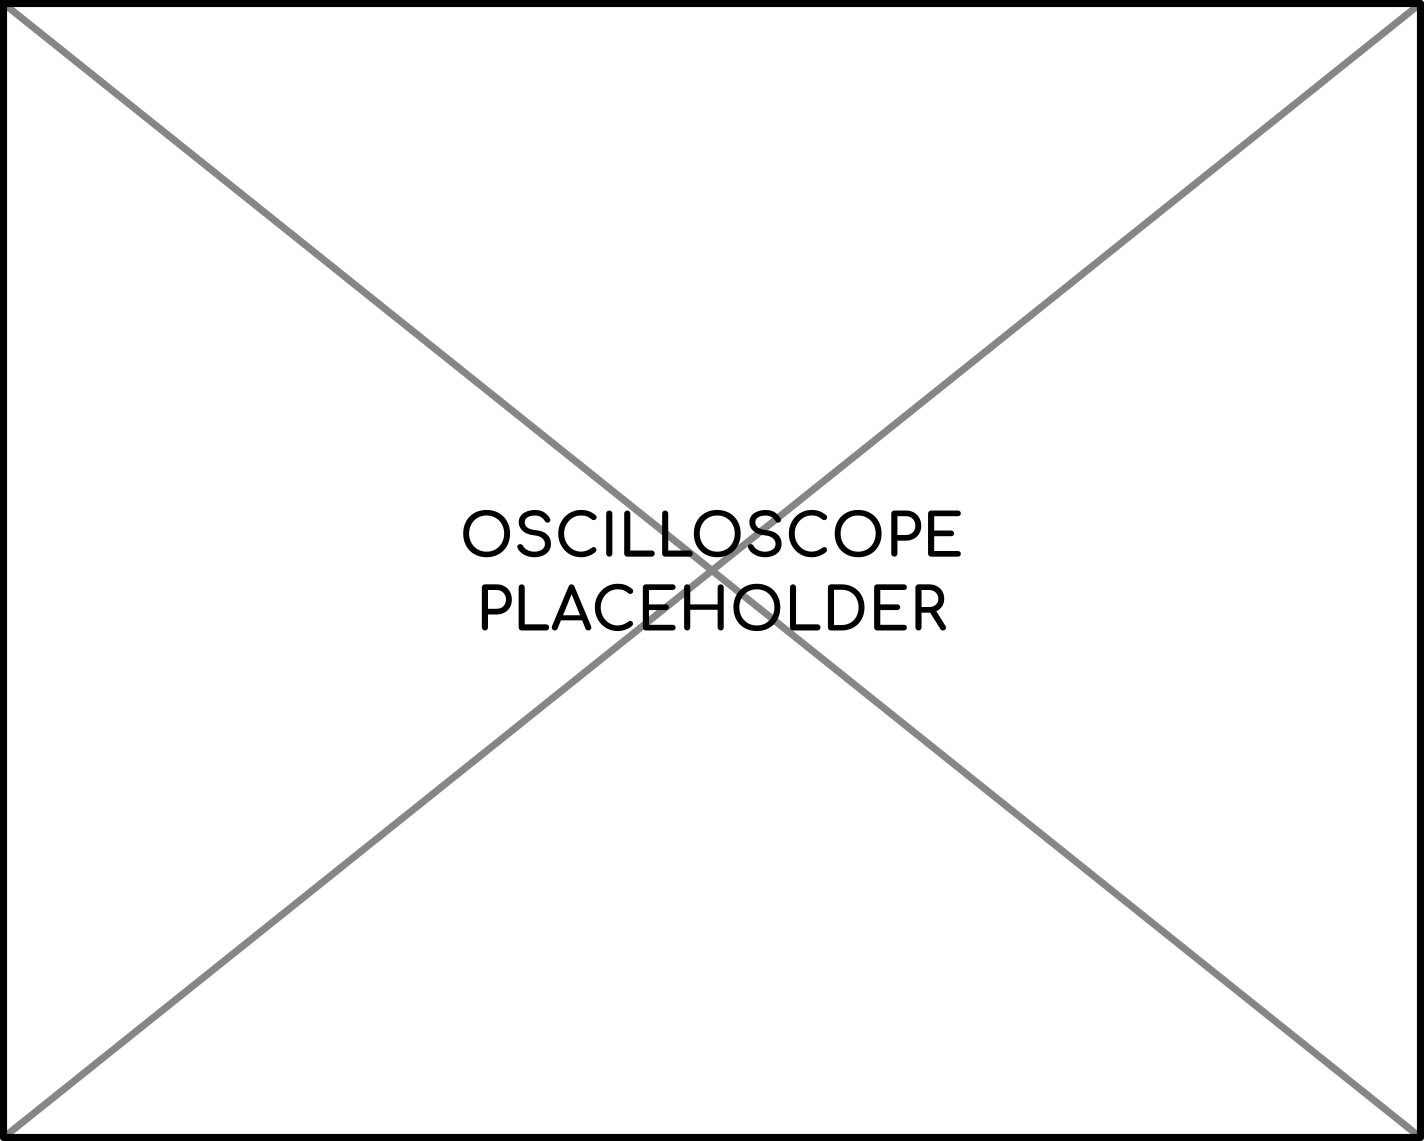
\includegraphics{misc/oscilloscope_placeholder.png}
        \caption{$V_{in}=+8\ V$}
        \label{acq_fourier_8V}
    \end{subfigure}

    \caption{Sinusoide ottenuta per diversi valori di $V_{in}$ nel dominio del tempo e
        della frequenza}
    \label{acq_sine}
\end{figure}

% osservazioni sulla bontà dell'onda

E la transcaratteristica tracciata tramite oscilloscopio risulta abbastanza simile a quella
teorica in figura.

\begin{figure}[H]
    \centering
    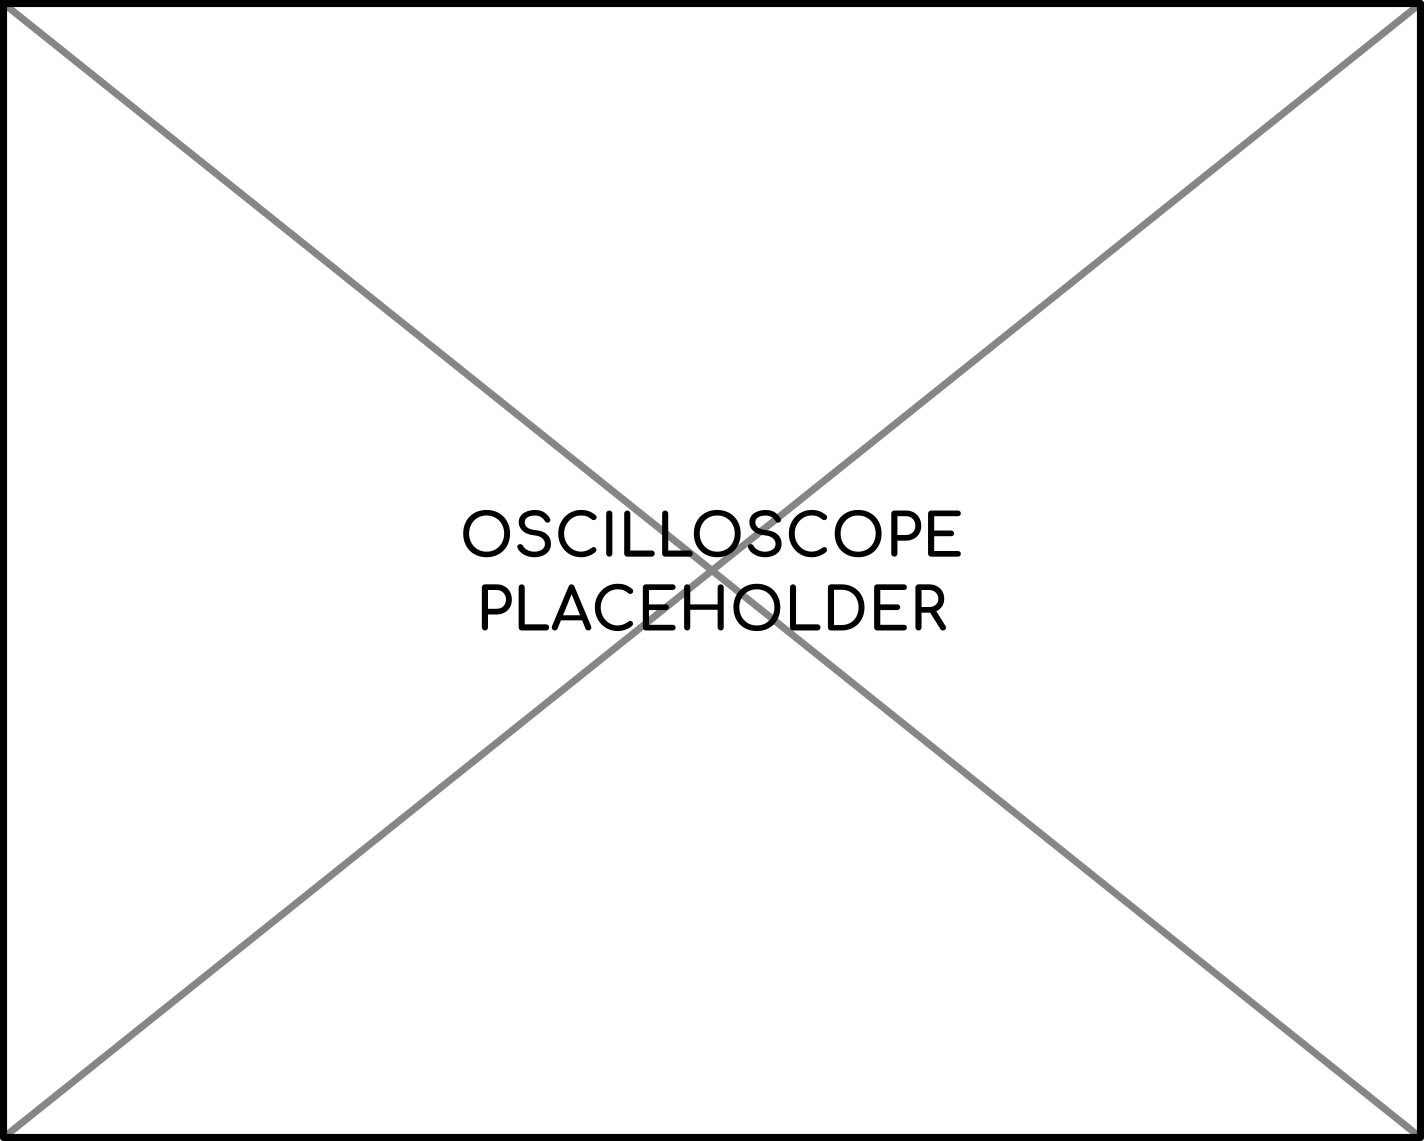
\includegraphics{misc/oscilloscope_placeholder.png}
    \caption{Transcaratteristica tracciata con l'oscilloscopio}
    \label{acq_sine_oscilloscope}
\end{figure}

%--------------------------------------------------------------------------------------------
